\subsection{Comparison of Epidemic Trajectories}
\label{sec:epidemic_comparison}

In this section, we analyze the macroscopic epidemic dynamics across the four proposed contact networks by performing 100 independent stochastic SIR simulations for each architecture.
Figure \ref{fig:sir_baseline} illustrates the resulting trajectories of susceptible, infected, and recovered populations, overlaid with the theoretical deterministic SIR curve calculated using Ordinary Differential Equations (ODEs).
As expected, the trajectories in the Mean Field (MF) and Erd\H{o}s-R\'enyi (ER) models closely align with the deterministic predictions, with average infection peaks of approximately 2,300 and 2,345 individuals, respectively.
The deterministic baseline provides a theoretical peak of 2,335 individuals occurring at Day 37.
Interestingly, the structured networks in Model 1 and Model 2 exhibit a significant departure from these homogeneous benchmarks.
In both Model 1 and Model 2, the infection peaks are notably higher and occur earlier than those predicted by the deterministic model and the ER network.
Specifically, the average stochastic peaks reached 2,634 individuals for Model 1 and 2,604 individuals for Model 2.
Furthermore, these structured models demonstrate a faster progression and an earlier termination of the outbreak compared to the MF and ER models.
While there are no substantial visual differences between the trajectories of Model 1 and Model 2 in this baseline scenario, both clearly highlight how demographic and institutional structures accelerate the initial phase of transmission.

\begin{figure}[H]
    \centering
    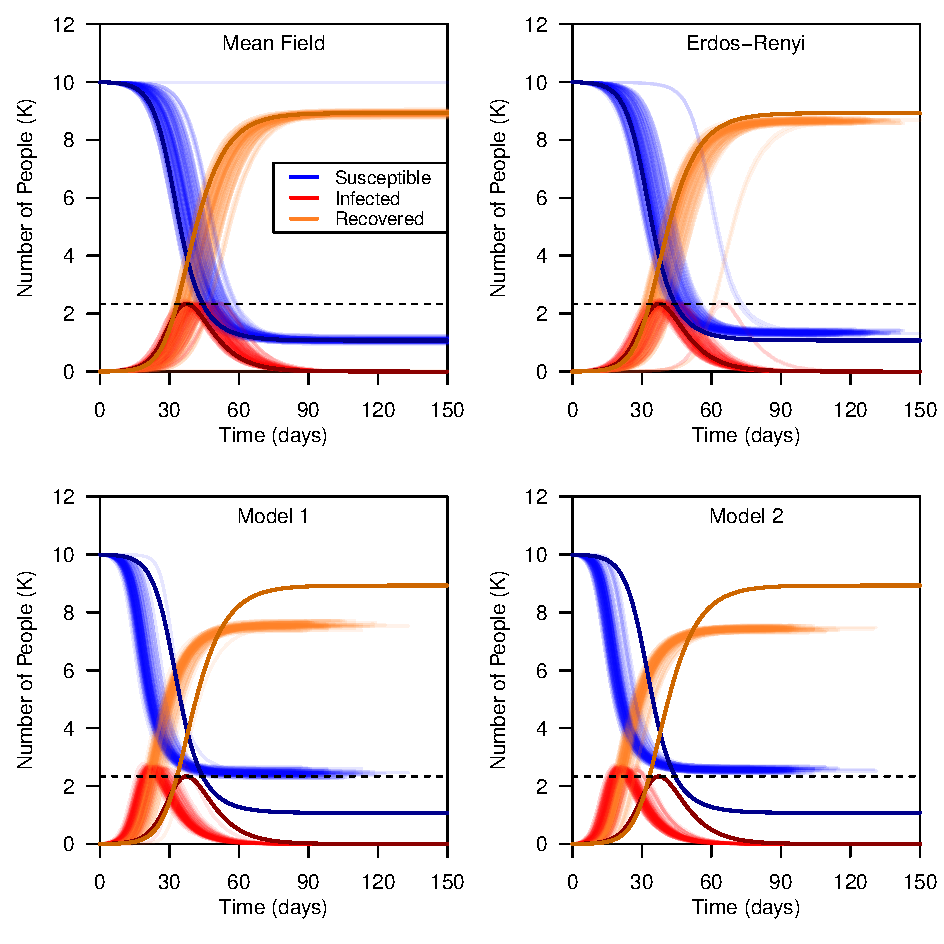
\includegraphics{figures/04_EpidemicModel/sir_baseline_r0_25.pdf}
    \caption{Stochastic SIR simulations across four baseline networks ($R_0 = 2.5$). The infection peaks in structured networks (Model 1 and Model 2) are higher and earlier than those in homogeneous models (Mean Field and Erd\H{o}s-R\'enyi) and the deterministic ODE prediction.}
    \label{fig:sir_baseline}
\end{figure}